\documentclass{beamer}
\usetheme{Montpellier}
\usecolortheme{beaver}
\usepackage{verbatim}	
\usepackage[square,sort]{natbib}
\usepackage{comment}
\usepackage{amsmath}
\usepackage{caption}


\setbeamerfont{footnote}{size=\tiny}
\setbeamerfont{footnote mark}{size=\tiny}
\setbeamerfont{caption}{size=\scriptsize}
\setbeamerfont{cite}{size=\tiny}


\title{Team 4 : Population Dynamics}

\author{Sajid Ali\inst{1} \& Brady Butler\inst{2}}	
\institute[NU] 
{\inst{1}%
	Applied Physics\\
	Northwestern University\\
	\inst{2}%	
	Physics\\
	University of Maine}
\date{\today}

% - Either use conference name or its abbreviation.
% - Not really informative to the audience, more for people (including
%   yourself) who are reading the slides online

%\subject{Theoretical Computer Science}
% This is only inserted into the PDF information catalog. Can be left
% out. 

% If you have a file called "university-logo-filename.xxx", where xxx
% is a graphic format that can be processed by latex or pdflatex,
% resp., then you can add a logo as follows:

\pgfdeclareimage[height=0.5cm]{university-logo}{pearc19}
\logo{\pgfuseimage{university-logo}}

% Delete this, if you do not want the table of contents to pop up at
% the beginning of each subsection:
\AtBeginSubsection[]
{
  \begin{frame}<beamer>{Outline}
    \tableofcontents[currentsection,currentsubsection]
  \end{frame}
}

% Let's get started
\begin{document}


\begin{frame}
  \titlepage
\end{frame}

\begin{frame}{Outline}
  \tableofcontents
  % You might wish to add the option [pausesections]
\end{frame}

% Section and subsections will appear in the presentation overview
% and table of contents.

\section{Lokta-Voletra!}
\begin{frame}{Predator-Prey Model}
	\begin{block}{}
		\begin{columns}[onlytextwidth,T]
			\column{\dimexpr\linewidth-40mm-10mm}
			\begin{itemize}
			\item $\frac{dM}{dt}=$
			\item $\frac{dW}{dt}=$
			\end{itemize}
			\column{40mm}
			\begin{figure}
				\hspace*{-1.1cm}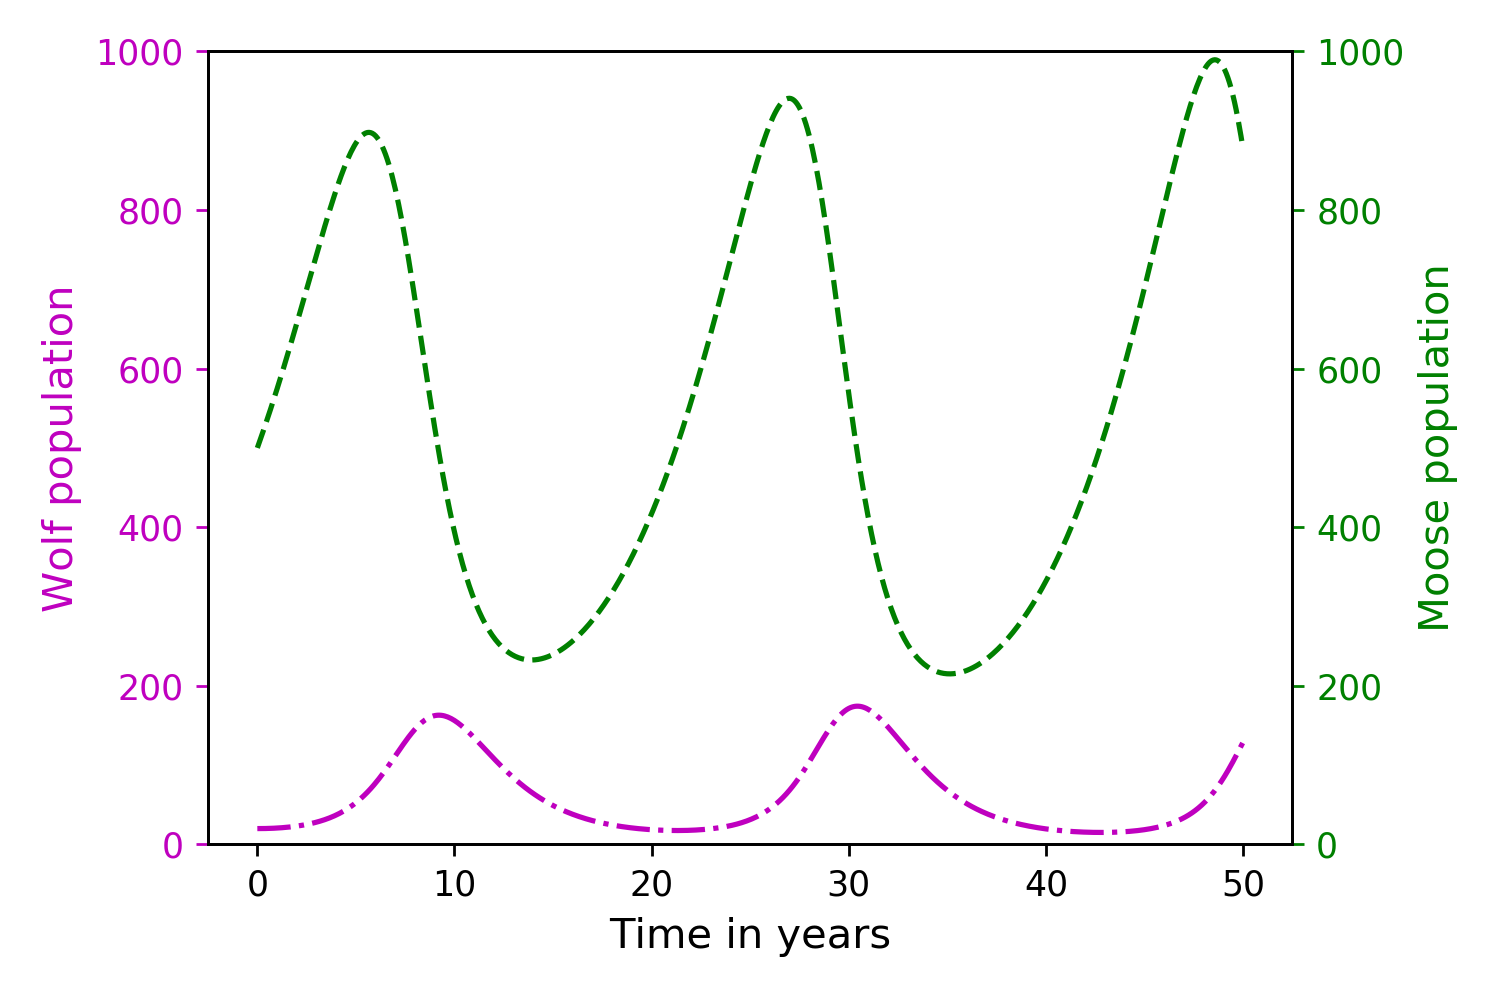
\includegraphics[width=60mm]{../plot_notebooks/sanity}
				\caption{Illustration of zone plate }
			\end{figure}
		\end{columns}
	\end{block}
\end{frame}




\section{Implementation}
\begin{frame}{Language \& Libraries!}
	\begin{itemize}
		\item some code was written.
	\end{itemize}
\end{frame}


\section{Results}
\begin{frame}{Results}
	\begin{itemize}
		\item Pretty plots!
	\end{itemize}
\end{frame}

\section{Conclusion}
\begin{frame}{Conclusion}
	\begin{itemize}
		\item And thus an important project was undertaken.
		\item Thank you to the organizers of PEARC19! 
	\end{itemize}
\end{frame}


% All of the following is optional and typically not needed. 
%\appendix
%\renewcommand*{\bibfont}{\small}
%\section{References}
%\begin{frame}[t, allowframebreaks]
%\frametitle{References}
%\bibliographystyle{alpha}
%\bibliography{fd}
%\end{frame}

\end{document}

